\documentclass[letterpaper]{article}
\usepackage{aaai}
\usepackage{url}
\usepackage{fullpage}
\usepackage{graphicx,curves}
\usepackage{amsmath}
\usepackage{amssymb}
%\usepackage{cmbright}
\usepackage{latexsym}
\usepackage{multirow}
\usepackage[algoruled,vlined,linesnumbered]{algorithm2e}
\usepackage{wrapfig}

\usepackage[bitstream-charter]{mathdesign}
%\renewcommand*\ttdefault{lmvtt}
\usepackage[T1]{fontenc}

\newtheorem{df}{Definition}
\newtheorem{notation}{Notation}
\newtheorem{theorem}{Theorem}
\newtheorem{lemma}{Lemma}[section]
\newtheorem{col}{Corollary}

\newcommand{\bt}{\begin{theorem}\em}
\newcommand{\et}{\end{theorem}}
\newcommand{\Qed}{$\blacksquare$}
\newcommand{\qed}{$\Box$}
\newcommand{\proof}{{\bf Proof. }}
\newcommand{\nin}{\noindent}
\newcommand{\bea}{\begin{eqnarray}}
\newcommand{\eea}{\end{eqnarray}}
\newcommand{\bdf}{\begin{df}\em}
\newcommand{\edf}{\end{df}}
\newcommand{\ben}{\begin{enumerate}}
\newcommand{\een}{\end{enumerate}}
\newcommand{\ie}{\item}
\newcommand{\dist}{\operatorname{dist}}
\newcommand{\avg}{\operatorname{avg}}

\newcommand{\citea}[1]{\citeauthor{#1} (\citeyear{#1})}

\numberwithin{equation}{section}
\numberwithin{theorem}{section}
\numberwithin{lemma}{section}
\numberwithin{df}{section}

\setcounter{secnumdepth}{3} %% this gives us back SECTION NUMBERS!


\title{Exceeding Human Intelligence in a Non-playable Character}

\nocopyright

\author{Joe Template \and Jane Example \\
Department of Computing Science \\ University of Alberta \\
Edmonton, Alberta, T6G 2E8, Canada \\
{\tt $\{$jtemplate$\mid$jexample$\}$@ualberta.ca}}


\begin{document}

\maketitle

\begin{abstract}
Introduce and motivate the problem. State the main idea of your solution approach and highlights of its evaluation.
\end{abstract}

\section{Introduction}

Informally introduce and motivate your problem here. 

\section{Problem Formulation}

Define the problem formally, including the performance criteria motivated by the introduction. The reader needs to know how to assess your approach's success or failure.

\section{Related Work}

Review related research and discuss its shortfalls with respect to the problem in the previous section. 

\section{Proposed Approach}

Describe your ideas for the proposed approach informally at first. Show how the proposed approach addresses the shortfalls of the related research that you discussed above. Then describe the approach formally and precisely enough to be reproduced by an independent researcher.

If you decide to use pseudocode (e.g., Algorithm~\ref{alg:fAlg})\footnote{Reproduced with permission from work by~\citea{flow}.}, make sure you complement it with a plain English description. Additionally hand trace your pseudocode line by line (make sure you refer to the line numbers in your pseudo-code) on a simple example.

\begin{algorithm*}[t]
\DontPrintSemicolon
\label{alg:fAlg}
\caption{Real-time Q-learning with lookahead $(\gamma, r, p, T)$}

initialize $Q_1$ to uniformly random values in $[0,1]$\;
\For{$t = 1,2, \dots, T$}
{
determine the amount of deliberation: $n_t \leftarrow \Delta(s_t)$ \; \label{al:amountOfDeliberation} 
set probe length: $m_t \leftarrow \lfloor \sqrt{n_t} \rfloor$ \; \label{al:probeLength}
number of probes: $k_t \leftarrow \lfloor \sqrt{n_t} \rfloor$ \; \label{al:probeNumber}
%
initialize enhanced state-action return estimates: $Q'_t \leftarrow Q_t$ \;
%
\For{$a \in A$\label{al:actionLoop}}
{
%
\For{$i = 1,\dots,k_t$\label{al:probeLoop}}
{
$s'_1 \leftarrow s_t$ \;\label{al:firstState}
$\gamma_1 \leftarrow 1$ \;
%
\For{$j = 1,\dots,m_t$\label{al:mActionLoop}}
{
select probe action: $a'_j \leftarrow \begin{cases}
a & \text{if $j=1$} \\ 
\arg \max_{a' \in A} Q'_t(s'_j,a') & \text{otherwise.} 
\end{cases}$ \; \label{al:selectProbeAction}
imagine the next state: $s'_{j+1} \leftarrow \Lambda(s'_j,a'_j)$ \;\label{al:applyProbeAction}
imagine the reward to be collected: $r'_j \leftarrow r(s'_j,a'_j)$ \;\label{al:collectProbeReward}
adjust the discount factor $\gamma_{j+1} \leftarrow \gamma_j \gamma$ \;
}
imagine the residual reward $r'_{m_t+1} \leftarrow \max_{a \in A} Q'_t(s'_{m_t+1},a)$ \;\label{al:residualReward}
%
\For{$j = 1,\dots,m_t$\label{al:probeUpdateLoop}}
{
update $Q'_t(s'_j,a'_j) \leftarrow (1-\alpha_t) Q'_t(s'_j,a'_j) + \alpha_t
\sum_{x = j}^{{m_t}+1} \gamma_x r'_x$ \;\label{al:learningProbe}
adjust discount factor: $\gamma_x \leftarrow \gamma_x / \gamma, x \in \{j+1,\dots,m_t+1\}$\;
}
}
}
execute the action: $a_t \leftarrow \arg \max^{\epsilon_t}_{a \in A} Q'_t(s_t,a)$ \;\label{al:actionSelect}\label{al:actionExecute}
observe the resulting state $s_{t+1}$ \;
%
update the return estimate using the collected reward and the new state: $Q_{t+1}(s_t,a_t) \leftarrow (1-\alpha_t) Q_t(s_t,a_t) + \alpha_t \left[ r(s_t,a_t) + \gamma \max_{a \in A} Q_t(s_{t+1},a) \right]$ \; \label{al:learningQ}
}
\end{algorithm*}

End this section formulating your hypothesis. For instance, ``my algorithm converges faster than X but uses more memory than Y under conditions A,B,C". Link your hypothesis to the motivation of the problem you gave earlier in the paper. For instance, if your hypothesis is about fast real-time operation then you should link it to the requirements of the problem at hand described earlier in the paper. 

\section{Theoretical Analysis}

Discuss expected properties of your algorithm. For instance, what is the run-time complexity in time and space? Under what assumptions is your algorithm guaranteed to find a solution? If it is a learning algorithm, under which conditions will it converge?

\section{Empirical Evaluation}

Support your hypothesis formulated above. First describe your empirical testbed in enough detail for an independent researcher to reproduce. Then describe all parameters of your algorithm as applied to the testbed. Finally present the results.

Do not be shy to list negative results as well --- they still improve our understanding of the field. Make sure your describe your experimental set up in enough detail for other researchers to replicate your work.

A solid empirical study not only offers some findings but also sheds light on how confident we should be about them. This can be accomplished through statistical tests (e.g., the T-test) and/or confidence intervals (e.g., Figure~\ref{fig:convPC}).

\begin{figure*}[t]
\begin{center}
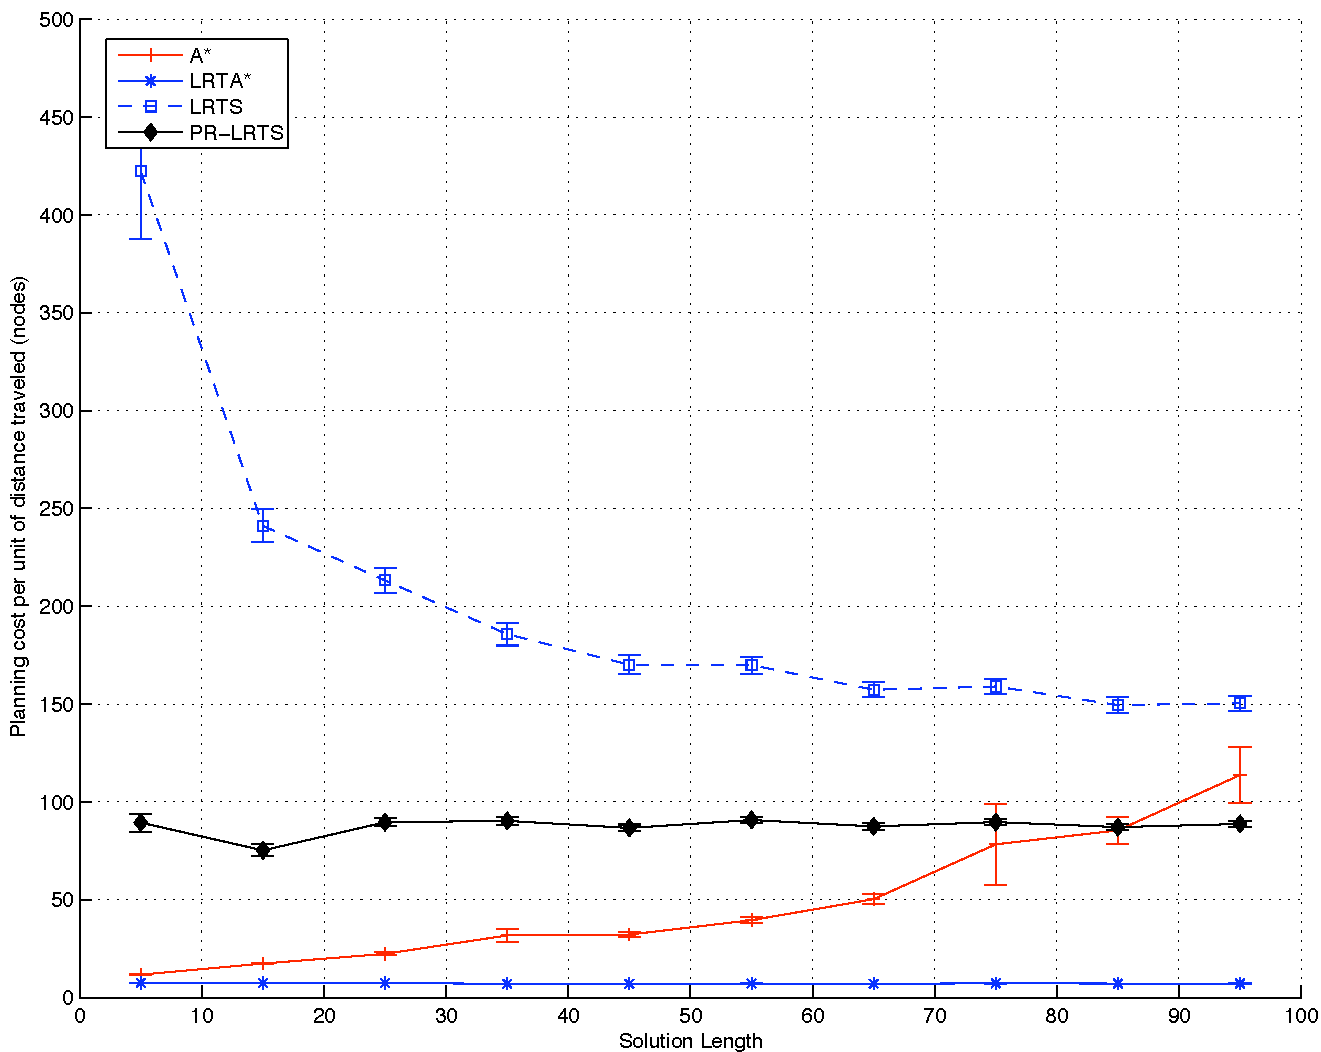
\includegraphics[width=\textwidth]{convPC.pdf}
\caption{\small Planning cost of various algorithms during convergence on initially unknown maps. Problems are bucketed according to their difficulty. Each of the ten buckets contains $100$ random path-planning problems.}\label{fig:convPC}
\end{center}
\end{figure*}

Complement your figures with compact and readable tables (e.g., Table~\ref{tab:PRLRTS-cummulative}). 

\begin{table}[t]
\caption{\small Typical results averaged over $50$ convergence runs on $10$ maps. The average shortest path length is $59.6$. Reproduced with permission from work by~\citea{Bulitko:05b}.}\label{tab:PRLRTS-cummulative}
\vspace{0.1cm}
{\small \begin{center}
\begin{tabular}{c|c|c|c}
\hline
 Algorithm & 1st move time & Conv. travel & Subopt. \\ \hline
A* & 5.01 ms & 186 & 0.0\% \\
LRTA* & 0.02 ms & 25,868 &  0.0\% \\
LRTS & 0.93 ms & 555 &  2.07\% \\
{\bf PR-LRTS} & {\bf 0.95 ms} & {\bf 345} & {\bf 2.19\%} \\
\hline
\end{tabular}
\end{center}}
\end{table}



\section{Discussion}

Discuss your results with respect to the hypotheses you formulated and the demands of the problem at hand. Do not be shy to admit that you do not understand some of the results you obtained. Leave them as open questions for further research. 

\section{Future Work}

Describe possible extensions (e.g., if you were to take on this project as your thesis work).

\section{Conclusions}

Refresh the reader on the problem at hand, motivation, shortfalls of the previous work, ideas of your new algorithm and the results of the empirical study. Briefly re-state the contributions your paper makes here. 


\section*{Acknowledgments}

Acknowledge any help you already received. 

\bibliography{projectReport}
\bibliographystyle{aaai}

\end{document}
